\chapter{Effectiveness of QUBO splitting}\label{sec:qsplitres}

This chapter analyzes the effectiveness of the \texttt{QSplitSampler}. 
Specifically, we will examine a straightforward and easily visualized case study in Section \ref{sec:maxcut}, followed by a comprehensive series of tests to evaluate the algorithm's general effectiveness in Section \ref{sec:qsplittest}.

\section{Test case: Maximum-Cut problem}\label{sec:maxcut}

To evaluate \texttt{QSplitSampler} in a controlled environment, the first context examined was its application to the Maximum-Cut problem.

\subsection{Maximum-Cut}

The Maximum-Cut problem involves dividing the vertices of a graph into two subsets, $S$ and $T$, such that the number of edges between nodes in $S$ and nodes in $T$ is maximized.

Consider a graph like the one in Figure \ref{fig:maxcut}. 
Subset $S$ consists of the white nodes, and subset $T$ consists of the black nodes. 
Figure \ref{fig:maxcutset} highlights all and only the edges between $S$ and $T$.

\begin{figure}[H]
    \centering
    \begin{subfigure}[b]{0.48\textwidth}
        \centering
        \begin{tikzpicture}
            \node[circle, fill=white, draw=black, inner sep=2pt, label=above:$A$] (A) at (0,2) {};
            \node[circle, fill=black, draw=black, inner sep=2pt, label=above:$B$] (B) at (2,2) {};
            \node[circle, fill=white, draw=black, inner sep=2pt, label=below:$C$] (C) at (2,0) {};
            \node[circle, fill=black, draw=black, inner sep=2pt, label=below:$D$] (D) at (0,0) {};
            \node[circle, fill=black, draw=black, inner sep=2pt, label=above:$E$] (E) at (-1.5,1) {};
            
            \draw[red, thick] (A) -- (B);
            \draw[red, thick] (B) -- (C);
            \draw[red, thick] (C) -- (D);
            \draw[red, thick] (D) -- (A);
            \draw[red, thick] (A) -- (E);
            \draw[black, thick] (E) -- (D);
        
            \draw[blue, thick] ($(A)+(0.75,0.5)$) -- ($(C)+(0.75,-0.75)$) -- ($(C)+(-0.75,-0.75)$) -- ($(A)+(-0.75,0.5)$);
        \end{tikzpicture}
        \caption{Maximum-Cut graph.}
        \label{fig:maxcut}
    \end{subfigure}
    \hfill
    \begin{subfigure}[b]{0.48\textwidth}
        \centering
        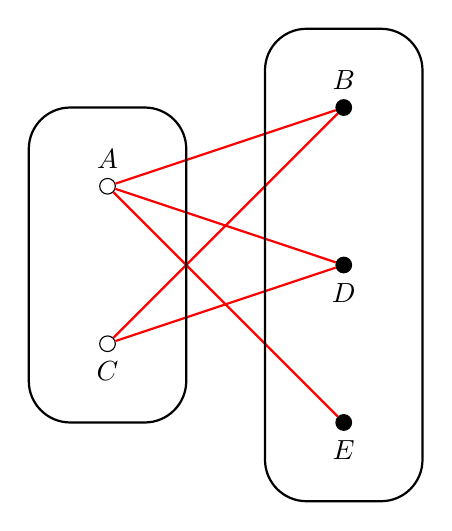
\begin{tikzpicture}
            \node[circle, fill=white, draw=black, inner sep=2pt, label=above:$A$] (A) at (0,3) {};
            \node[circle, fill=white, draw=black, inner sep=2pt, label=below:$C$] (C) at (0,1) {};
            
            \node[circle, fill=black, draw=black, inner sep=2pt, label=above:$B$] (B) at (3,4) {};
            \node[circle, fill=black, draw=black, inner sep=2pt, label=below:$D$] (D) at (3,2) {};
            \node[circle, fill=black, draw=black, inner sep=2pt, label=below:$E$] (E) at (3,0) {};
            
            \draw[red, thick] (A) -- (B);
            \draw[red, thick] (A) -- (E);
            \draw[red, thick] (A) -- (D);
            \draw[red, thick] (C) -- (B);
            \draw[red, thick] (C) -- (D);
            
            \draw[black, thick, rounded corners=15pt] (-1,0) rectangle (1,4);
            \draw[black, thick, rounded corners=15pt] (2,-1) rectangle (4,5);
        \end{tikzpicture}
        \caption{Rearranged graph in $S$ and $T$.}
        \label{fig:maxcutset}
    \end{subfigure}
    \caption{Maximum-Cut (a) and subdivision into subsets (b).}
\end{figure}

\paragraph{Desired Characteristics} In the case illustrated in Figure \ref{fig:maxcut}, it is easily verifiable that it is impossible to find an assignment of $S$ and $T$ that produces more than five edges.

However, the solution is not unique. 
If we associate $1$ with the white nodes and $0$ with the black nodes, two five-edge solutions are: 
\begin{itemize}
    \item $\{A=1,B=0,C=1,D=0,E=0\}$,
    \item $\{A=0,B=1,C=0,D=1,E=1\}$.
\end{itemize}

The non-uniqueness of the solution presents a challenge during the optimization process, as different sections of the problem might guide towards complementary assignments, leading to inconsistent aggregated results.

\subsection{Results}

The test problem is illustrated in Figure \ref{fig:maxcut_test}, consisting of a graph with eight nodes, corresponding to eight variables. 
\texttt{QSplitSampler} was configured to solve problems of size two using the QPU, meaning that the QPU receives problems that are $\frac{1}{16}$ of the total size.

In this case, partitioning is unnecessary, as the QPU can directly solve problems of this size. 
The utility of this experiment lies in providing an initial measure of error.

\begin{figure}[H]
    \centering
    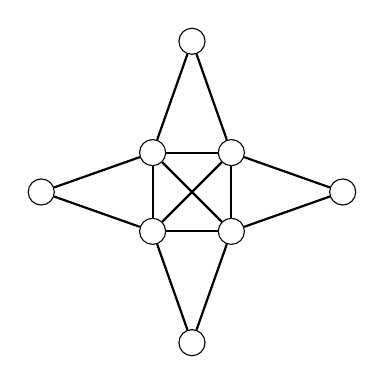
\begin{tikzpicture}
        \node[circle, draw=black] (A) at (0,1.914) {};
        \node[circle, draw=black] (B) at (1.914,3.828) {};
        \node[circle, draw=black] (C) at (3.828,1.914) {};
        \node[circle, draw=black] (D) at (1.914,0) {};
        \node[circle, draw=black] (E) at (1.414,1.414) {};
        \node[circle, draw=black] (F) at (1.414,2.414) {};
        \node[circle, draw=black] (G) at (2.414,2.414) {};
        \node[circle, draw=black] (H) at (2.414,1.414) {};

        \draw[black, thick] (A) -- (E);
        \draw[black, thick] (A) -- (F);
        \draw[black, thick] (B) -- (F);
        \draw[black, thick] (B) -- (G);
        \draw[black, thick] (C) -- (G);
        \draw[black, thick] (C) -- (H);
        \draw[black, thick] (D) -- (H);
        \draw[black, thick] (D) -- (E);
        \draw[black, thick] (E) -- (F);
        \draw[black, thick] (E) -- (H);
        \draw[black, thick] (E) -- (G);
        \draw[black, thick] (F) -- (G);
        \draw[black, thick] (F) -- (H);
        \draw[black, thick] (H) -- (G);
    \end{tikzpicture}
    \caption{Graph used to test Maximum-Cut.}
    \label{fig:maxcut_test}
\end{figure}

The results obtained are summarized in Table \ref{tab:maxcut}.

\begin{table}[H]
    \centering
    \begin{tabular}{cccc}
        \toprule
        \multicolumn{2}{c}{\texttt{QSplitSampler}} & \multicolumn{2}{c}{Direct resolution} \\
        Time (s) & Solution & Time (s) & Solution \\
        \midrule
        18.15 & 0.8 & 5.02 & 0        
    \end{tabular}
    \caption{\texttt{QSplitSampler} executed on \ref{fig:maxcut_test}.}
    \label{tab:maxcut}
\end{table}

The time required to process the problem is expressed in seconds and includes the following components: 
\begin{itemize} 
    \item Processing on the CPU, which, in the case of a direct solution, consists only of initializing the data structure; 
    \item Network transfer, to send the problem to quantum solvers;
    \item Processing on the QPU, to produce the solution. 
\end{itemize}

The solution is presented by normalizing the values within the range $[0, 1]$. 
Since these are minimization problems, $0$ corresponds to the optimal solution.

\paragraph{Time Analysis} The time required to solve \ref{fig:maxcut_test} with \texttt{QSplitSampler} is 3.6 times greater than that of a direct resolution. 
This increase is not only due to the CPU processing required by the partitioning and aggregation strategy but also the higher number of requests made to the quantum solver. 
Although the problems are relatively small, it is necessary to transmit the data to D-Wave's cloud infrastructure, wait for processing, and then forward the result. 
This computational overhead might become marginal for instances where quantum acceleration is substantial, but it significantly impacts the resolution of ``small'' problems.

\paragraph{Quality of Results} From a performance perspective, \texttt{QSplitSampler} produced results that were significantly worse compared to direct resolution. 
However, it is important to contextualize these results.

\texttt{QSplitSampler} provided a response of $0.8$, a value closer to the maximum assignment than to the minimum. 
For the tests conducted, this represents an upper bound on the error made in producing a solution. 
The poor quality of the response could be due to multiple optimal solutions, all equivalent from an algorithmic standpoint but leading to final assignments that are inconsistent with the original problem.

\section{Extensive testing}\label{sec:qsplittest}

To evaluate the performance of \texttt{QSplitSampler} in a broader context than that described in Section \ref{sec:maxcut}, random problems were generated using D-Wave's libraries. 
The problems considered represent complete graphs, and while they do not represent SVMs, they preserve their structure and information density.

Working with complete graphs increases the likelihood of having multiple optimal assignments. 
Intuitively, this occurs because the problem has more data to combine to converge to the same objective function value.

In Section \ref{sec:multivar}, the results obtained with problems of $64$ and $128$ variables are reported, while in Section \ref{sec:yqsplit}, general considerations on \texttt{QSplitSampler} are presented, analyzing the reasons behind the obtained results.

\subsection{64 and 128 Variables Problems}\label{sec:multivar}

Tables \ref{tab:64var} and \ref{tab:128var} respectively present the results for problems with $64$ and $128$ variables. The table columns provide the following information, with all times expressed in seconds: 
\begin{itemize} 
    \item \emph{Cut Dim}: the size of the \texttt{QSplitSampler} subproblem solved by the QPU; 
    \item \emph{CPU time}: the time required by \texttt{QSplitSampler} to produce a solution, which includes: 
    \begin{itemize} 
        \item The time taken for minor embedding computation; 
        \item The time for network transfer to D-Wave's cloud infrastructure; 
        \item The time spent on classical architecture processing (division and aggregation of results). 
    \end{itemize} 
    \item \emph{QPU time}: the time spent on the QPU; 
    \item \emph{Solution}: the value of the best solution, normalized to $[0, 1]$, produced by \texttt{QSplitSampler}; 
    \item \texttt{QPUSampler}: the solution produced by directly solving the problem on the QPU. 
\end{itemize}

\begin{table}[H]
    \centering
    \begin{tabular}{cccc|cc}
        \toprule
        \multicolumn{4}{c}{\texttt{QSplitSampler}} & \\
        Cut Dim         & CPU time & QPU time & Solution & \texttt{QPUSampler} \\
        \midrule
        2               & 156.9    & 0.33     & 0.26     & 0        \\
        4               & 63.6     & 0.25     & 0.46     & 0        \\
        8               & 35.4     & 0.17     & 0.47     & 0        \\
        16              & 20.8     & 0.1      & 0.31     & 0        \\
        32              & 22.8     & 0.05     & 0.26     & 0        \\
        \bottomrule
    \end{tabular}
    \caption{Results for problems with 64 variables.}
    \label{tab:64var}
\end{table}

\begin{table}[H]
    \centering
    \begin{tabular}{cccc|c}
        \toprule
        \multicolumn{4}{c}{\texttt{QSplitSampler}} & \\
        Cut Dim         & CPU time & QPU time & Solution & \texttt{QPUSampler}  \\
        \midrule
        2               & 417.8    & 0.45     & 0.49     & 0        \\
        4               & 173.3    & 0.35     & 0.41     & 0        \\
        8               & 105.8    & 0.25     & 0.42     & 0        \\
        16              & 49.7     & 0.17     & 0.39     & 0        \\
        32              & 42       & 0.1      & 0.36     & 0        \\
        \bottomrule
    \end{tabular}
    \caption{Results for problems with 128 variables.}
    \label{tab:128var}
\end{table}

In both cases, the quality of the solution produced deviates significantly from the optimum, deteriorating between 25\% and 50\%. 
Furthermore, the lower limit of the error committed seems to increase as the problem size increases, stabilising at around 35\%.

Despite the suboptimal results, \texttt{QSplitSampler} maintains the desired behaviour regarding QPU usage. 
All reported values exceed 0.1 seconds, three times higher than the use of D-Wave's hybrid solver (Section \ref{sec:qpuusage}) for significantly larger problems.

However, despite the significant increase in the quantum component used to find the solution, the time required to transmit all the subproblems and aggregate the results remains dominant.

\subsection{General Observations}\label{sec:yqsplit}

Based on the results obtained, the following key considerations emerge: 
\begin{itemize} 
    \item The effectiveness of maximizing QPU usage as a resolution strategy; 
    \item The evident increase in solution time as \emph{cut dim} decreases. 
\end{itemize}

\paragraph{Performance} Although no clear relationship emerges between the parameters \texttt{QSplitSampler} and the quality of the solution produced, it is evident that an error of at least 25\% for small-sized problems is not acceptable. 
The poor performance is likely due to the search for complementary assignments, a case which is not currently addressed during execution but may warrant further analysis.

\paragraph{Solving Time} The increase in solution time as \emph{cut dim} decreases is considerable, raising the question of where most of the time is spent during execution. 
Understanding the bottleneck of the current implementation may allow for the development of a second, potentially more efficient version.

The methods used for subdivision and aggregation of subproblems are efficient enough not to have a significant impact on execution.

Likewise, the time required for transmission to the cloud infrastructure should not be so high as to slow down execution. 
However, how many subproblems are transferred remains to be verified. 
Although a single transmission may be negligible, extensive use of network resources could justify the observed behaviour.

To handle a problem with $2^a$ variables by sending subproblems of size $2^b$ to the QPU, where $a \geq b$, means transmitting a total of $3^{a-b}$ subproblems to the quantum solver. 
This calculation considers only the number of subproblems sent to the QPU. 
If the subproblems generated from the aggregation process are also considered, the total number of calls to the QPU would be $3^{a-b} + 3*(a-b)$.

Thus, for a problem with $128$ variables ($2^7$) and a \emph{cut dim} of $2$, the number of subproblems transmitted is at least: $3^{7-1}=3^6=729$.

Although \texttt{QSplitSampler} allows for handling problems larger than the QPU limits (Section \ref{sec:qpu-res}), the proposed methodology is insufficient for solving problems of the size discussed in Section \ref{sec:qsvm-res}. 
The version of SVM used generates a problem with $32,768$ ($2^{15}$) variables, calculated according to Equation \eqref{eq:nodesnum}. 
Even assuming a \emph{cut dim} of $64$ ($2^6$), the number of problems to be sent to the QPU would be at least $3^{15-6}=3^9=19,683$.
